% Diego Sebastián Aliaga Damián
% 2024200481M
% Tema 96: Fintech y financiamiento participativo (crowdfunding) en el Perú: oferta y condiciones
% Diapositivas (máximo 10, consigna 2.5). Las cifras usan \cifra{...} y las figuras salen de ../../salidas/figuras.
% BORRADOR ASISTIDO POR IA (2026-11-12): ensayar la exposición y ajustar el texto con tus palabras.

% ---------------------------------------------------------------- 1. Portada
% La franja inferior y los logos van en el fondo de la diapositiva (plantilla «background»): así se ubican bien
% tanto al proyectar como al imprimir dos diapositivas por hoja.
{
\setbeamertemplate{background}{%
  \begin{tikzpicture}
    \useasboundingbox (0,0) rectangle (\paperwidth,\paperheight);
    \fill[negro] (0,0) rectangle (\paperwidth,0.85cm);
    \fill[rojo] (0,0.85cm) rectangle (\paperwidth,0.95cm);
    \fill[amarillo] (0,0.95cm) rectangle (\paperwidth,0.985cm);
    \node[anchor=west, text=white, font=\scriptsize] at (0.6cm,0.42cm)
      {Universidad Nacional del Centro del Perú · Facultad de Economía · Escuela Profesional de Economía};
    \node[anchor=east, text=white, font=\scriptsize] at ($(\paperwidth,0.42cm)+(-0.6cm,0)$) {Huancayo, 2026-II};
    \draw[negro, line width=0.6pt] ($(\paperwidth,1.45cm)+(-3.75cm,0)$) -- ($(\paperwidth,\paperheight)+(-3.75cm,-0.55cm)$);
    \node[anchor=north] at ($(\paperwidth,\paperheight)+(-1.95cm,-0.5cm)$) {
\includegraphics[width=2.25cm]{logo_uncp.png}};
    \node[anchor=north] at ($(\paperwidth,\paperheight)+(-1.95cm,-3.15cm)$) {
\includegraphics[width=2.6cm]{logo_facultad.png}};
  \end{tikzpicture}}
\begin{frame}[plain,t]
  \vspace*{0.35cm}
  \begin{minipage}[t]{0.71\textwidth}
    {\color{rojo}\scriptsize\bfseries FINANZAS I \enspace|\enspace UNIDAD II \enspace|\enspace TEMA N.\textsuperscript{o}~96\par}
    \vspace{0.25cm}
    {\singuiones\color{negro}\bfseries\fontsize{15.5}{19}\selectfont Fintech y financiamiento participativo (crowdfunding) en el Perú: oferta y condiciones, 2022-2026\par}
    \vspace{0.12cm}
    {\color{rojo}\rule{2.6cm}{2.6pt}}\par\vspace{0.08cm}
    {\footnotesize\itshape\color{gris} Fintech and crowdfunding in Peru: Supply and financing terms, 2022-2026\par}
    \vspace{0.35cm}
    \begin{minipage}[t]{0.52\linewidth}
      \rotulo{Autor}\par{\small\bfseries Diego Sebastián Aliaga Damián}\par{\scriptsize Código 2024200481M}\par\vspace{0.2cm}
      \rotulo{Institución}\par{\scriptsize Universidad Nacional del Centro del Perú\\Facultad de Economía}
    \end{minipage}\hfill
    \begin{minipage}[t]{0.44\linewidth}
      \rotulo{Docente}\par{\scriptsize Dr. Ciro Iván Machacuay Meza}\par\vspace{0.2cm}
      \rotulo{Curso}\par{\scriptsize Finanzas I (055D), Unidad II}
    \end{minipage}
  \end{minipage}
\end{frame}
}

% ---------------------------------------------------------------- 2. Contexto y problema
\begin{frame}{Contexto y problema de investigación}
  \begin{columns}[t]
    \begin{column}{0.52\textwidth}
      \rotulo{¿Por qué estudiar el financiamiento participativo?}\par\vspace{0.15cm}
      \begin{itemize}\small
        \item El \textbf{financiamiento participativo financiero} (FPF) conecta, mediante una plataforma, a quienes buscan financiamiento con inversionistas.
        \item Está regulado desde el D.~U. N.\textsuperscript{o}~013-2020 y el reglamento de la SMV (2021), modificado en noviembre de 2025.
        \item El crédito tradicional es caro: la TEA bancaria a la pequeña y microempresa (hasta 360 días) subió de \dato{\cifra{teaBcosPyme2022}~\%} en 2022 a \dato{\cifra{teaBcosPyme2026}~\%} en 2026.
      \end{itemize}
    \end{column}
    \begin{column}{0.44\textwidth}
      \begin{tarjeta}{Problema}
        Solo circulan cifras anuales sueltas de prensa: no hay una caracterización de la oferta con datos oficiales y reproducibles.
      \end{tarjeta}
      \begin{destacada}{Pregunta de investigación}
        ¿Cómo es la oferta de FPF en el Perú entre 2022 y 2026 y cómo se comparan sus condiciones con las del crédito tradicional?
      \end{destacada}
    \end{column}
  \end{columns}
\end{frame}

% ---------------------------------------------------------------- 3. Objetivos e hipótesis
\begin{frame}{Objetivos e hipótesis}
  \begin{destacada}{Objetivo general}
    Caracterizar la oferta de financiamiento participativo financiero en el Perú (2022-2026) y comparar sus condiciones observables con las del crédito tradicional.
  \end{destacada}
  \vspace{-0.1cm}
  \begin{columns}[t]
    \begin{column}{0.235\textwidth}\begin{tarjeta}[equal height group=oe, fonttitle=\bfseries\scriptsize]{OE1 · Oferta}\scriptsize Plataformas, proyectos, montos y concentración.\end{tarjeta}\end{column}
    \begin{column}{0.235\textwidth}\begin{tarjeta}[equal height group=oe, fonttitle=\bfseries\scriptsize]{OE2 · Plataformas}\scriptsize Situación financiera y costo de intermediación.\end{tarjeta}\end{column}
    \begin{column}{0.235\textwidth}\begin{tarjeta}[equal height group=oe, fonttitle=\bfseries\scriptsize]{OE3 · Acceso}\scriptsize Colocación y monto por receptor, antes y después de 2025.\end{tarjeta}\end{column}
    \begin{column}{0.235\textwidth}\begin{tarjeta}[equal height group=oe, fonttitle=\bfseries\scriptsize]{OE4 · Comparación}\scriptsize Frente al crédito tradicional y límites de la comparación.\end{tarjeta}\end{column}
  \end{columns}
  \vspace{0.12cm}
  \begin{columns}[t]
    \begin{column}{0.32\textwidth}\scriptsize\dato{H1}\ El monto mensual es mayor tras la modificación del reglamento.\end{column}
    \begin{column}{0.32\textwidth}\scriptsize\dato{H2}\ La colocación difiere entre proyectos empresariales y personales.\end{column}
    \begin{column}{0.32\textwidth}\scriptsize\dato{E1}\ ¿Se asocian los cambios del monto con los de las tasas tradicionales?\end{column}
  \end{columns}
\end{frame}

% ---------------------------------------------------------------- 4. Fuentes de datos y extracción
\begin{frame}{Fuentes de datos y extracción automatizada}
  \begin{columns}[t]
    \begin{column}{0.315\textwidth}
      \begin{tarjeta}[equal height group=fu, halign title=center]{BCRP}\centering
        {\color{rojo}\bfseries BCRPData · API REST}\par\scriptsize 10 series mensuales: TEA pyme y consumo de bancos y cajas, TAMN e IPC\par\vspace{0.05cm}\textbf{JSON}
      \end{tarjeta}
    \end{column}
    \begin{column}{0.315\textwidth}
      \begin{tarjeta}[equal height group=fu, halign title=center]{SMV}\centering
        {\color{rojo}\bfseries OData · API}\par\scriptsize Estados financieros de las sociedades administradoras, 23 trimestres\par\vspace{0.05cm}\textbf{JSON}
      \end{tarjeta}
    \end{column}
    \begin{column}{0.315\textwidth}
      \begin{tarjeta}[equal height group=fu, halign title=center]{SMV}\centering
        {\color{rojo}\bfseries SIMV · \textit{scraping}}\par\scriptsize Proyectos y montos por plataforma y mes: \cifra{plataformasAutorizadas} plataformas × 69 meses\par\vspace{0.05cm}\textbf{HTML (ASP.NET)}
      \end{tarjeta}
    \end{column}
  \end{columns}
  \vspace{0.15cm}
  \rotulo{Flujo de trabajo}\par\vspace{0.1cm}
  \centering
  \begin{tikzpicture}[
      paso/.style={draw=negro, fill=white, rounded corners=2pt, align=center, font=\tiny, minimum height=0.85cm, text width=2.15cm, inner sep=2pt},
      clave/.style={paso, fill=negro, text=white},
      flecha/.style={-{Stealth[length=1.8mm]}, thick, color=rojo}]
    \node[clave] (a) {\textbf{Fuentes oficiales}\\BCRP · SMV};
    \node[paso, right=0.32cm of a] (b) {\textbf{01 y 02 · Python}\\API y \textit{scraping}};
    \node[paso, right=0.32cm of b] (c) {\textbf{03 · Limpieza}\\panel \cifra{filasPanel} × \cifra{columnasPanel}};
    \node[paso, right=0.32cm of c] (d) {\textbf{04 · Análisis}\\8 tablas y 4 figuras};
    \node[clave, fill=rojo, draw=rojo, right=0.32cm of d] (e) {\textbf{Auditoría}\\pruebas y cotejo en vivo};
    \foreach \x/\y in {a/b, b/c, c/d, d/e} \draw[flecha] (\x) -- (\y);
  \end{tikzpicture}\par\vspace{0.12cm}
  {\scriptsize \dato{\cifra{solicitudesHTTP}} solicitudes con HTTP 200 \enspace·\enspace cobertura del portal \dato{\cifra{coberturaPct}~\%} \enspace·\enspace pausas de 3 s \enspace·\enspace SHA-256 y crudos sin editar\par}
\end{frame}

% ---------------------------------------------------------------- 5. Demostración en vivo
\begin{frame}[fragile]{Demostración en vivo de la extracción (3 minutos)}
  \begin{columns}[t]
    \begin{column}{0.6\textwidth}
      \begin{tarjeta}{Paso 1 · Scraping en vivo del portal de la SMV}
\verb|python codigo\02_scraping_web.py --demo|\par\vspace{0.05cm}
        {\footnotesize 3 solicitudes (unos 15 s): consulta un mes de la plataforma líder y lo compara con la base entregada.}
      \end{tarjeta}
      \begin{tarjeta}{Paso 2 · Cotejo con las fuentes oficiales}
\verb|python codigo\auditoria.py --en-vivo|\par\vspace{0.05cm}
        {\footnotesize Elige 10 filas al azar y verifica cada valor contra la API del BCRP y el portal de la SMV.}
      \end{tarjeta}
    \end{column}
    \begin{column}{0.36\textwidth}
      \begin{destacada}{Qué se verifica}
        \begin{itemize}\footnotesize
          \item Código HTTP y validación de la tabla devuelta
          \item Datos en vivo iguales a los entregados
          \item Los crudos no se modifican
          \item Pausas y agente de usuario identificable
        \end{itemize}
      \end{destacada}
    \end{column}
  \end{columns}
\end{frame}

% ---------------------------------------------------------------- 6. OE1: oferta
\begin{frame}{Oferta: crecimiento rápido y muy concentrado}
  \begin{columns}[c]
    \begin{column}{0.61\textwidth}
      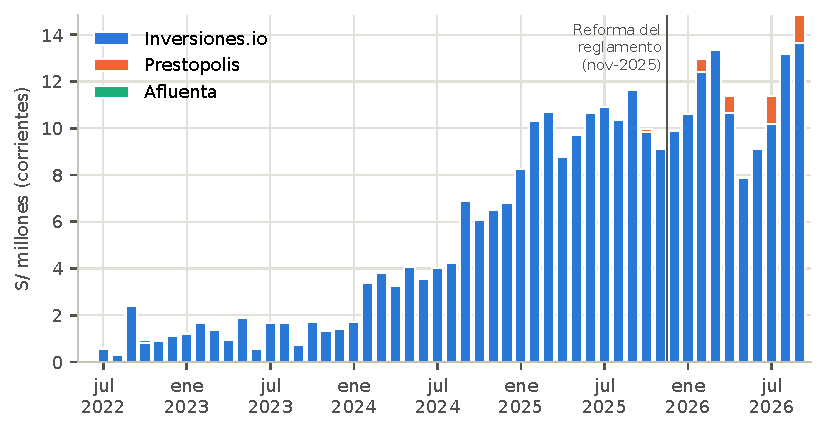
\includegraphics[width=\linewidth]{f1_monto_mensual_por_plataforma.pdf}
      \fuente{\cifra{tituloF1}. Fuente: SMV (SIMV).}
    \end{column}
    \begin{column}{0.36\textwidth}
      \begin{tarjeta}[halign title=center]{Lectura}
        \linea{Concentración}{Solo \cifra{plataformasConFinanciamiento} de \cifra{plataformasAutorizadas} sociedades financiaron; \cifra{nombreLider} reúne el \cifra{participacionLider}~\% del monto.}
        \linea{Crecimiento}{S/~\cifra{monto2022} M en 2022 → S/~\cifra{monto2025} M en 2025; IHH de \cifra{hhi2025}.}
        \linea{2026 (ene-sep)}{S/~\cifra{monto2026} M, \cifra{varMonto2026}~\% más que en 2025.}
        \linea{Perfil}{Empresarial: \cifra{partEmp2026}~\% del monto en 2026.}
      \end{tarjeta}
    \end{column}
  \end{columns}
\end{frame}

% ---------------------------------------------------------------- 7. OE2: plataformas
\begin{frame}{Plataformas: pequeñas y solo una rentable}
  \begin{columns}[c]
    \begin{column}{0.57\textwidth}
      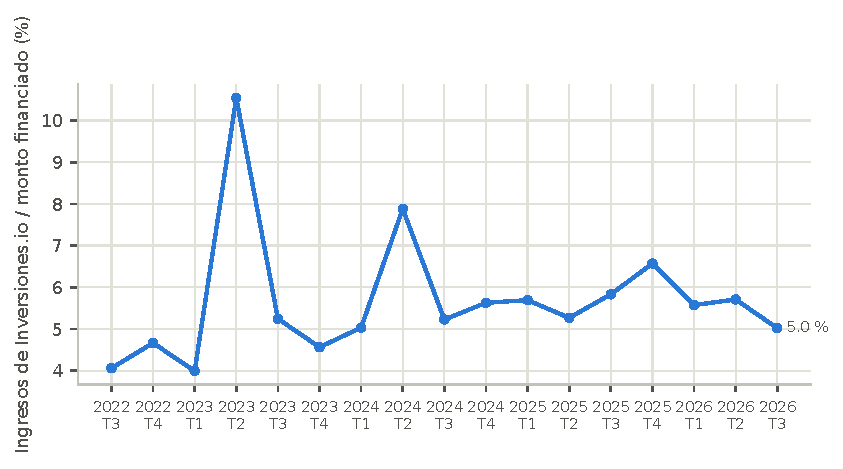
\includegraphics[width=\linewidth]{f4_costo_intermediacion_implicito.pdf}
      \fuente{\cifra{tituloF4}. Fuente: SMV (API OData y SIMV).}
    \end{column}
    \begin{column}{0.4\textwidth}
      \begin{tarjeta}[halign title=center]{Lectura}
        \linea{Escala}{La líder cerró 2025 con activos de S/~\cifra{activoLider2025} mil, mientras su mercado financió S/~\cifra{monto2025} M.}
        \linea{Rentabilidad}{ROA anualizado de la líder: \cifra{roaLider2025}~\% (2025); las demás perdieron en \cifra{aniosOtrasPerdida} de \cifra{aniosOtras} años.}
        \linea{Ingresos / monto}{Mediana trimestral de \cifra{costoMediana}~\%.}
      \end{tarjeta}
      \begin{destacada}{Ojo}
        Es lo que retiene la plataforma, \textbf{no} la tasa que paga el receptor.
      \end{destacada}
    \end{column}
  \end{columns}
\end{frame}

% ---------------------------------------------------------------- 8. OE3: acceso y reforma
\begin{frame}{Acceso por receptor y la reforma de 2025}
  \begin{columns}[t]
    \begin{column}{0.48\textwidth}
      \begin{tarjeta}[equal height group=hh]{H2 · Colocación por tipo de receptor}
        Empresariales \dato{\cifra{colocacionEmp}~\%} y personales \dato{\cifra{colocacionPer}~\%} ($z=\cifra{hDosZ}$).\par\smallskip
        Pero el \cifra{pctEmpresarialPrincipal}~\% de los empresariales es de \cifra{nombreLider} y el \cifra{pctPersonalPrincipal}~\% de los personales, de \cifra{principalPersonal}.\par\smallskip
        Dentro de la líder: prueba de Fisher, $p\cifra{hDosFisherPRel}$.\par\medskip
        {\color{rojo}\bfseries → Refleja el modelo de negocio, no el receptor.}
      \end{tarjeta}
    \end{column}
    \begin{column}{0.48\textwidth}
      \begin{tarjeta}[equal height group=hh]{H1 · Monto antes y después de la reforma}
        Mediana mensual: S/~\cifra{hUnoMedianaAntes} M → \dato{S/~\cifra{hUnoMedianaDespues} M} ($p\cifra{hUnoPRel}$).\par\smallskip
        Pero \cifra{placeboN} cortes ficticios previos también dan $p\cifra{placeboPMaxRel}$; el crecimiento interanual bajó de \cifra{interanualAntes}~\% a \cifra{interanualDespues}~\%, y \cifra{mesesSobreTendencia} de \cifra{mesesDespues} meses superan la tendencia previa.\par\medskip
        {\color{rojo}\bfseries → Mayor, pero no atribuible a la norma.}
      \end{tarjeta}
    \end{column}
  \end{columns}
\end{frame}

% ---------------------------------------------------------------- 9. OE4: crédito tradicional
\begin{frame}{Frente al crédito tradicional}
  \begin{columns}[c]
    \begin{column}{0.59\textwidth}
      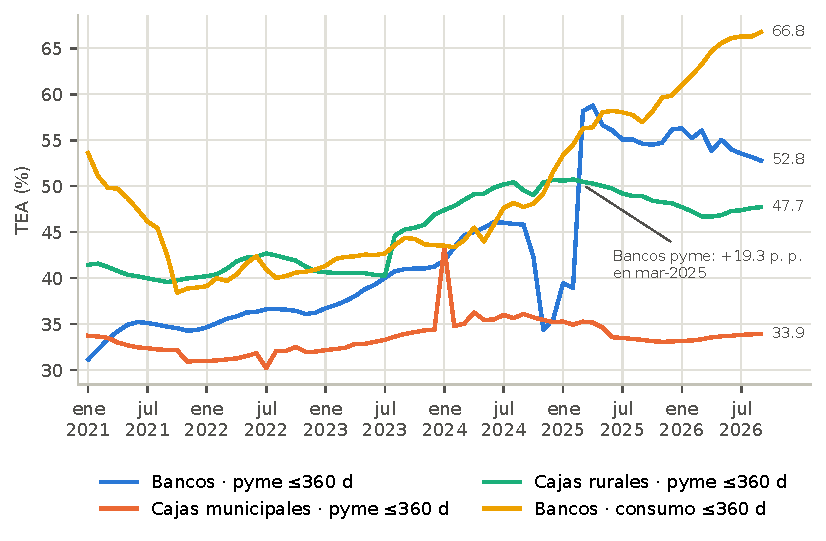
\includegraphics[width=\linewidth]{f3_tasas_credito_tradicional.pdf}
      \fuente{\cifra{tituloF3}. Fuente: BCRP (BCRPData).}
    \end{column}
    \begin{column}{0.38\textwidth}
      \begin{tarjeta}[halign title=center]{Lectura}
        \linea{Cajas}{Municipales: \cifra{teaCmacPymeMin}-\cifra{teaCmacPymeMax}~\%; rurales: \cifra{teaCracPymeMin}-\cifra{teaCracPymeMax}~\%.}
        \linea{Bancos pyme}{Salto de \cifra{saltoTEA} p.~p. en marzo de 2025.}
        \linea{E1}{Sin asociación con el FPF (\cifra{eUnoN} comparadores, $p_{\min}=\cifra{eUnoPMin}$).}
      \end{tarjeta}
      \begin{destacada}{Límite}
        La SMV no publica la tasa ni el plazo de cada operación: el precio del FPF \textbf{no es comparable}.
      \end{destacada}
    \end{column}
  \end{columns}
\end{frame}

% ---------------------------------------------------------------- 10. Conclusiones
\begin{frame}{Conclusiones e implicancias}
  \begin{destacada}[halign title=center]{¿Qué encontramos?}
    \centering El FPF creció de S/~\cifra{monto2022} M a S/~\cifra{monto2025} M al año, pero es un mercado \textbf{pequeño en participantes y muy concentrado}, sin información pública sobre su precio.
  \end{destacada}
  \vspace{-0.1cm}
  \begin{columns}[t]
    \begin{column}{0.235\textwidth}\begin{tarjeta}[equal height group=cc, fonttitle=\bfseries\scriptsize]{1. Oferta}\scriptsize Una plataforma concentra casi todo el monto.\end{tarjeta}\end{column}
    \begin{column}{0.235\textwidth}\begin{tarjeta}[equal height group=cc, fonttitle=\bfseries\scriptsize]{2. Plataformas}\scriptsize Préstamos a empresas; solo la líder es rentable.\end{tarjeta}\end{column}
    \begin{column}{0.235\textwidth}\begin{tarjeta}[equal height group=cc, fonttitle=\bfseries\scriptsize]{3. Acceso y reforma}\scriptsize Pesa el modelo de negocio; el aumento tras 2025 no es atribuible a la norma.\end{tarjeta}\end{column}
    \begin{column}{0.235\textwidth}\begin{tarjeta}[equal height group=cc, fonttitle=\bfseries\scriptsize]{4. Precio}\scriptsize Sin tasa ni plazo por operación, no se compara con la banca.\end{tarjeta}\end{column}
  \end{columns}
  \vspace{0.05cm}
  \begin{columns}[c]
    \begin{column}{0.8\textwidth}\footnotesize
      \rotulo{Implicancia}\par La SMV debería publicar la tasa, el plazo y la morosidad de cada operación para evaluar si el FPF ofrece mejores condiciones que la banca y las cajas.
    \end{column}
    \begin{column}{0.16\textwidth}\centering\qrcode[height=1.45cm]{\repositorio}\par{\tiny Repositorio}\end{column}
  \end{columns}
\end{frame}
